
\newpage
%%%%%%%%%%%%%%%%%%%%%%%%%%%%%%%%%%%%%%%%%%%%%%%%%%%%%%%%%%%%%%%%%%%%%%%%%%%%%%%%
%%%%%%%%%%%%%%%%%%%%%%%%%%%%%%%%%%%%%%%%%%%%%%%%%%%%%%%%%%%%%%%%%%%%%%%%%%%%%%%%
\section{Dançando fora do ritmo ou da métrica?}
\index{Musicalidade!Fora do ritmo}
\index{Musicalidade!Fora da métrica}

Existe uma confusão no uso da expressão ``dançar fora do ritmo'',
pois comumente é usado para se referir a ``dançar fora da métrica'';
é claro que um \hyperref[sec:pos:Ritmo]{\textbf{ritmo}} está sujeito a uma \hyperref[def:Metrica]{\textbf{métrica}}, 
e se falamos que estamos fora do ritmo,
podemos também nos estar referindo a  dançar fora da métrica, 
porem isto é uma imprecisão que poucas vesses conseguirá
uma correta transmissão de nossas ideias.
Para entender melhor esta diferença descreveremos ambos casos


\begin{definition}[Dançar fora da métrica:]
Dançar fora da \hyperref[def:Metrica]{\textbf{métrica}}
 implica que dada uma porção de peça musical,
nossos movimentos estão sendo executados sem 
\hyperref[sec:musicalidadeinfmutua]{\textbf{informação mutua}} com a métrica
dessa porção de música.

A métrica de uma porção de música nos da informação da distribuição
dos tempos dos compassos, e também qual será o acento métrico de cada um desses tempos.
\end{definition}

\begin{definition}[Dançar fora do ritmo:]
\label{def:fora-do-ritmo}
Dançar fora do \hyperref[sec:pos:Ritmo]{\textbf{ritmo}}
implica que dada uma voz dentro de uma porção de peça musical,
nossos movimentos estão sendo executados sem 
\hyperref[sec:musicalidadeinfmutua]{\textbf{informação mutua}} com a 
informação rítmica dessa voz nessa porção de música.

O ritmo de uma voz na música, 
se refere à distribuição temporal na execução dos sons e a sua proporção na duração
destes.
\end{definition}

Para entender melhor a Definição \ref{def:fora-do-ritmo}, a 
Figura \ref{fig:fora-do-ritmo-0-1} mostra a pauta de uma melodia executada por um bandolim, 
representando a voz escolhida para nossa dança; 
na parte inferior da pauta está representada a parte rítmica dessa melodia.
Assim, nesse caso, dançar fora do ritmo implica dançar fora do ritmo do bandolim;
é dizer, que entre esse ritmo e nossa dança existe pouca ou nula informação mutua.
Pelo que se acompanhamos essa melodia executando um ritmo regular como 
\Vier \Acht \Acht~(tum tic tic), com o tum no tempo forte;
nos dançaríamos dentro da métrica da melodia,
mas fora do ritmo dela. 
Assim, a frase ``dançar fora da métrica'' é a que expressa melhor o fato de estar descompromissado com os tempos
e os acentos nos compassos. 
\begin{figure}[!h]
    \centering 
    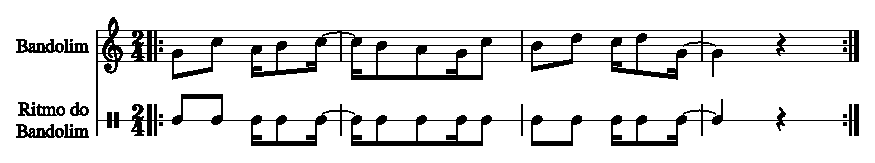
\includegraphics[width=0.99\textwidth]{chapters/cap-musicalidade/fora-do-ritmo-0-1.eps}
    \caption{Dançando respeitando a métrica.}
    \label{fig:fora-do-ritmo-0-1}
\end{figure}

\begin{example}[Dançando dentro da métrica:]
A Figura \ref{fig:fora-do-ritmo-com} mostra três casos onde um dançarino
executa bases rítmicas dentro da métrica da música. 
Neste caso a música  tem um \hyperref[subsec:compassobinario]{\textbf{compasso binário simples}}.
\begin{itemize}
\item Na primeira base rítmica se utiliza um ritmo repetitivo e regular \Vier \Acht \Acht~(tum tic tic),
com o mesmo período e acentuação estabelecido pela métrica. 
\item A segunda base rítmica, ao igual que a primeira, cumpre a métrica da música,
só que agora usa um ritmo \Vier \Vier~(tum tum).
\item A terceira base rítmica, ao igual que as anteriores, cumpre a métrica da música,
só que agora usa um ritmo \Acht. \Sech \Vier~(bum a tum).
\end{itemize}
\end{example}

\begin{figure}[!h]
    \centering 
    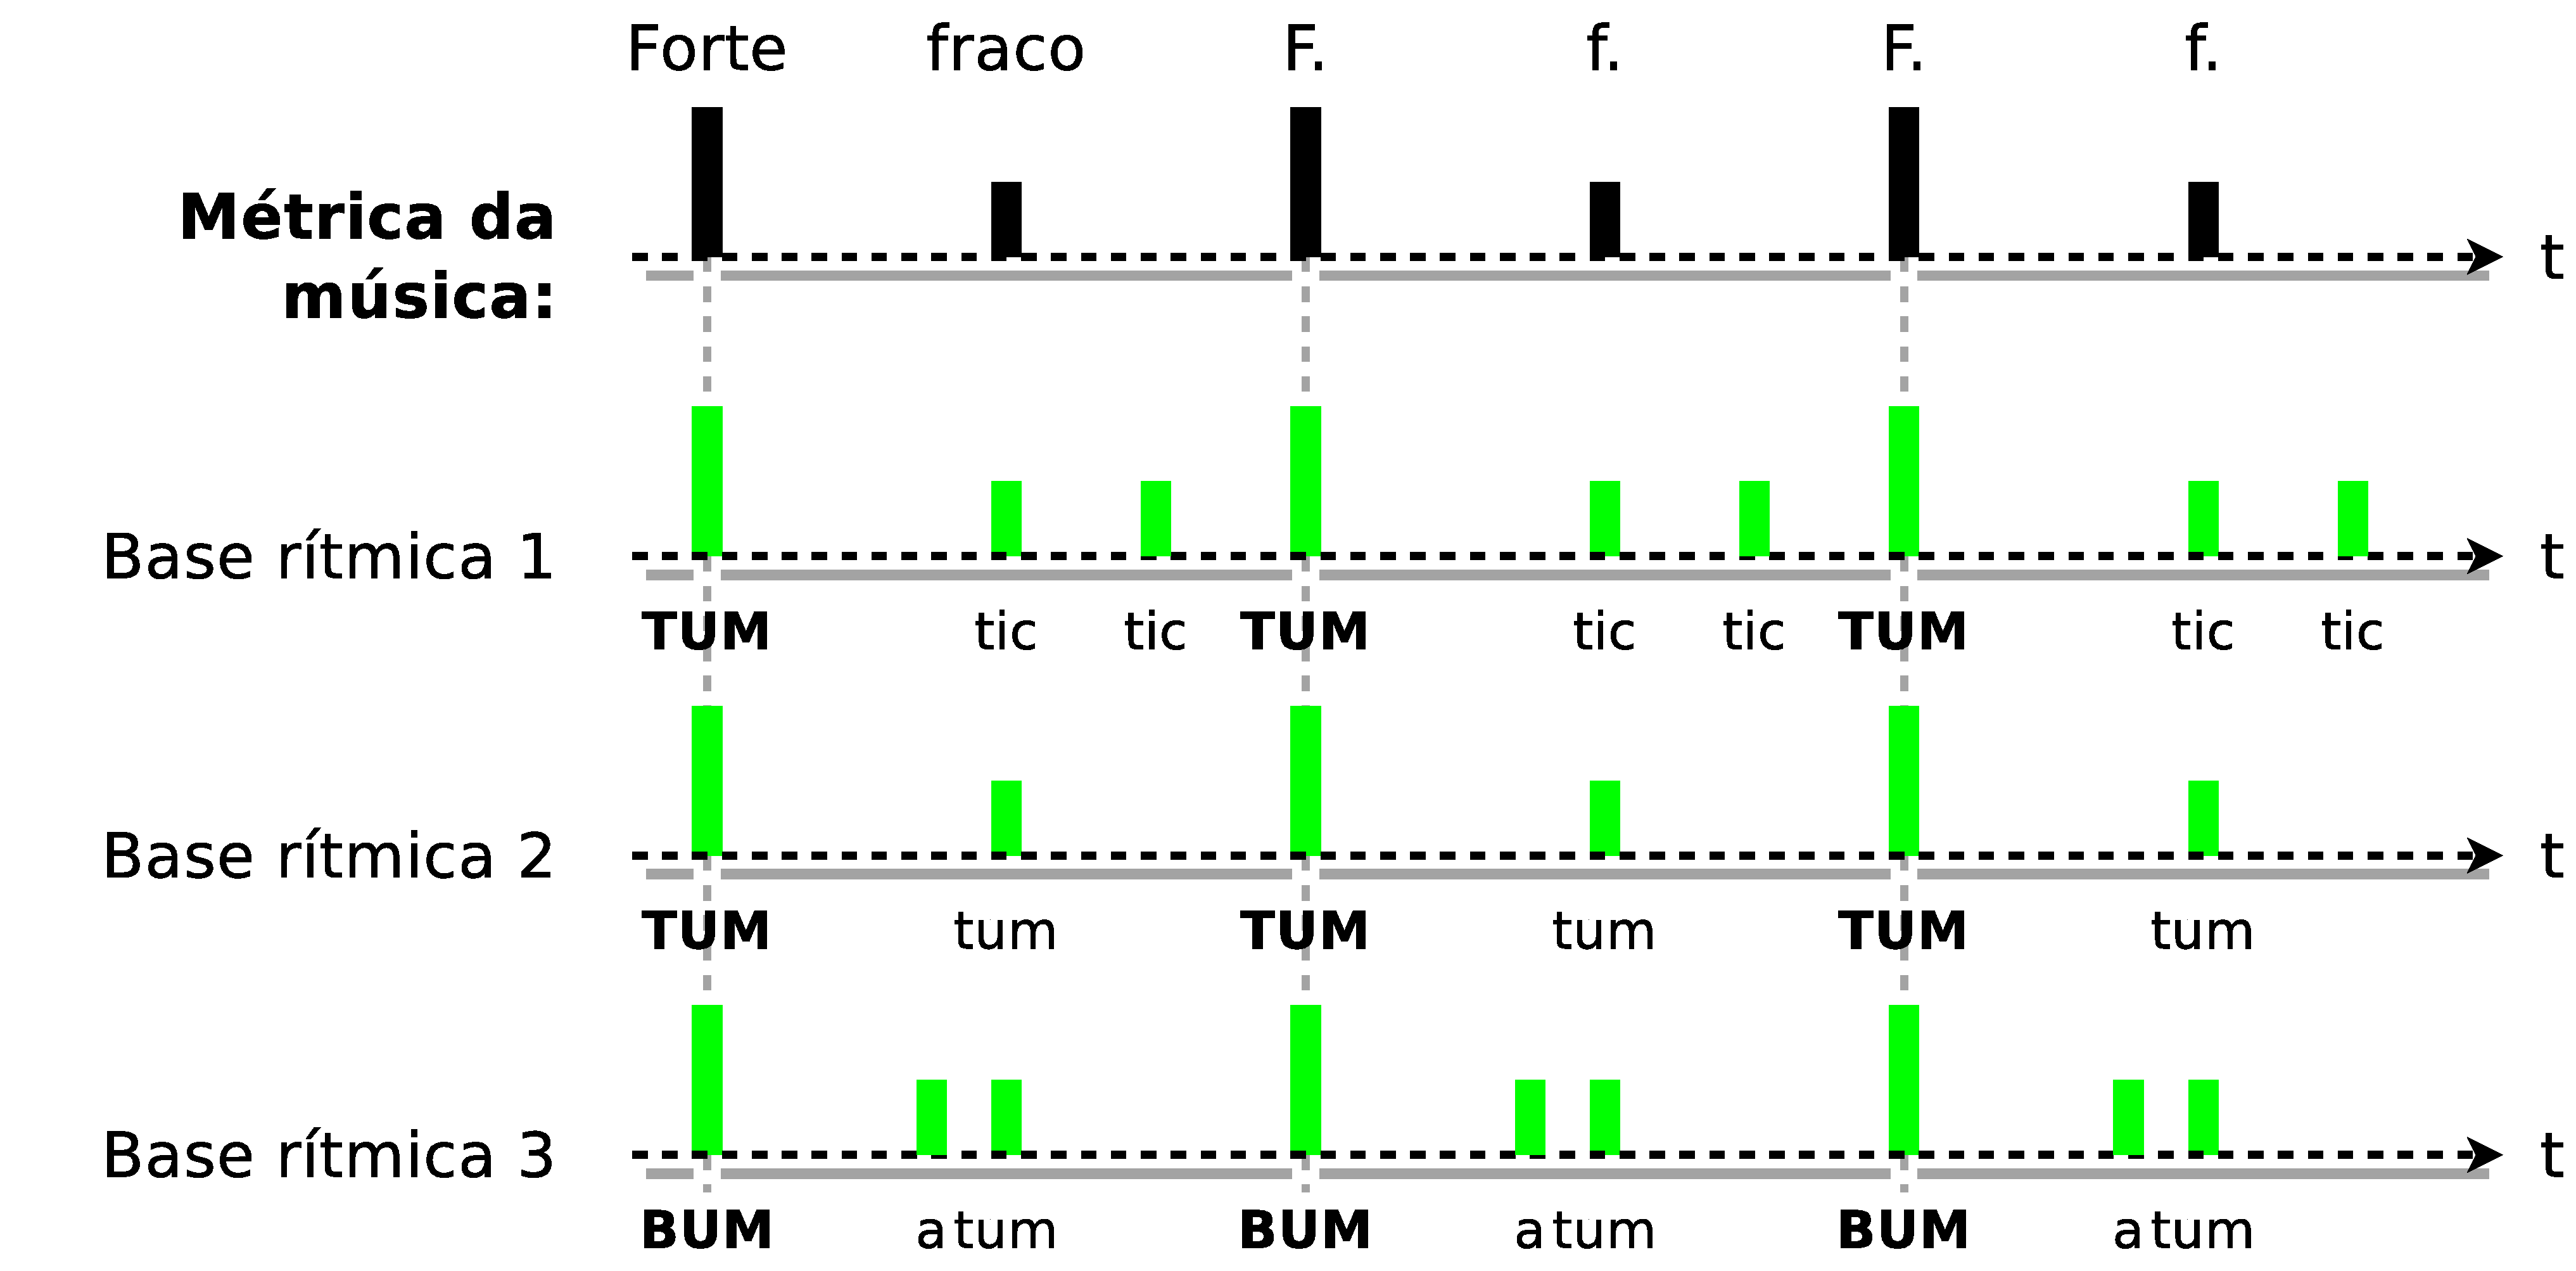
\includegraphics[width=0.99\textwidth]{chapters/cap-musicalidade/fora-do-ritmo-com.eps}
    \caption{Dançando respeitando a métrica.}
    \label{fig:fora-do-ritmo-com}
\end{figure}

\begin{tcbattention}
\begin{itemize}
\item Mais detalhes sobre como \hyperref[subsec:perceberTF1]{\textbf{reconhecer os tempos fortes}} 
e fracos podem ser vistos na Seção \ref{subsec:perceberTF1}.
\item Mais detalhes sobre o que é \hyperref[subsec:dancametrica]{\textbf{dançar na métrica}}, 
podem ser vistos na Seção \ref{subsec:dancametrica}.
\item Mais detalhes sobre o que é \hyperref[subsec:dancaritmo]{\textbf{dançar no ritmo}}, 
podem ser vistos na Seção \ref{subsec:dancaritmo}.
\item Outros temas relativos a dançar no ritmo são: 
\hyperref[subsec:dancamelodia]{\textbf{dançar na melodia}} e
\hyperref[subsec:dancamusica]{\textbf{dançar na música}},
que podem ser vistos nas Seções \ref{subsec:dancamelodia} e \ref{subsec:dancamusica},
respetivamente.
\end{itemize}
\end{tcbattention}

\begin{example}[Dançando fora da métrica:]
\label{ex:fora-do-ritmo:2}
A Figura \ref{fig:fora-do-ritmo-sem} mostra três casos 
onde um dançarino executa bases rítmicas fora da métrica da música,
Neste caso as três bases rítmicas utilizam um ritmo repetitivo e regular \Vier \Acht \Acht~(tum tic tic),
e a música  tem um \hyperref[subsec:compassobinario]{\textbf{compasso binário simples}}.
\begin{itemize}
\item A primeira base rítmica é executada com um \hyperref[sec:Andamento]{\textbf{andamento}} com
a mesma velocidade que a métrica da música; 
porem os movimentos tem uma desfasagem (atraso) na acentuação. 
Muito provavelmente produzido porque o dançarino esperou sentir o pulso musical para logo atuar,
e não predizer lho e atuar. 
\item A segunda base rítmica também é executada com um \hyperref[sec:Andamento]{\textbf{andamento}} com
a mesma velocidade que a métrica da música; 
porem os movimentos são acentuados em lugares aleatórios, 
pelo que não se está acompanhando a acentuação métrica.
\item A terceira base rítmica é executada com um \hyperref[sec:Andamento]{\textbf{andamento}} incorreto;
assim, mesmo que ele acentue seus passos de forma regular, estes sempre estarão mal colocados,
produto da desfasagem provocada pelas diferentes velocidades de andamento,
neste caso o dançarino tem um andamento de maior velocidade.
\end{itemize}
\end{example}
\begin{figure}[!h]
    \centering 
    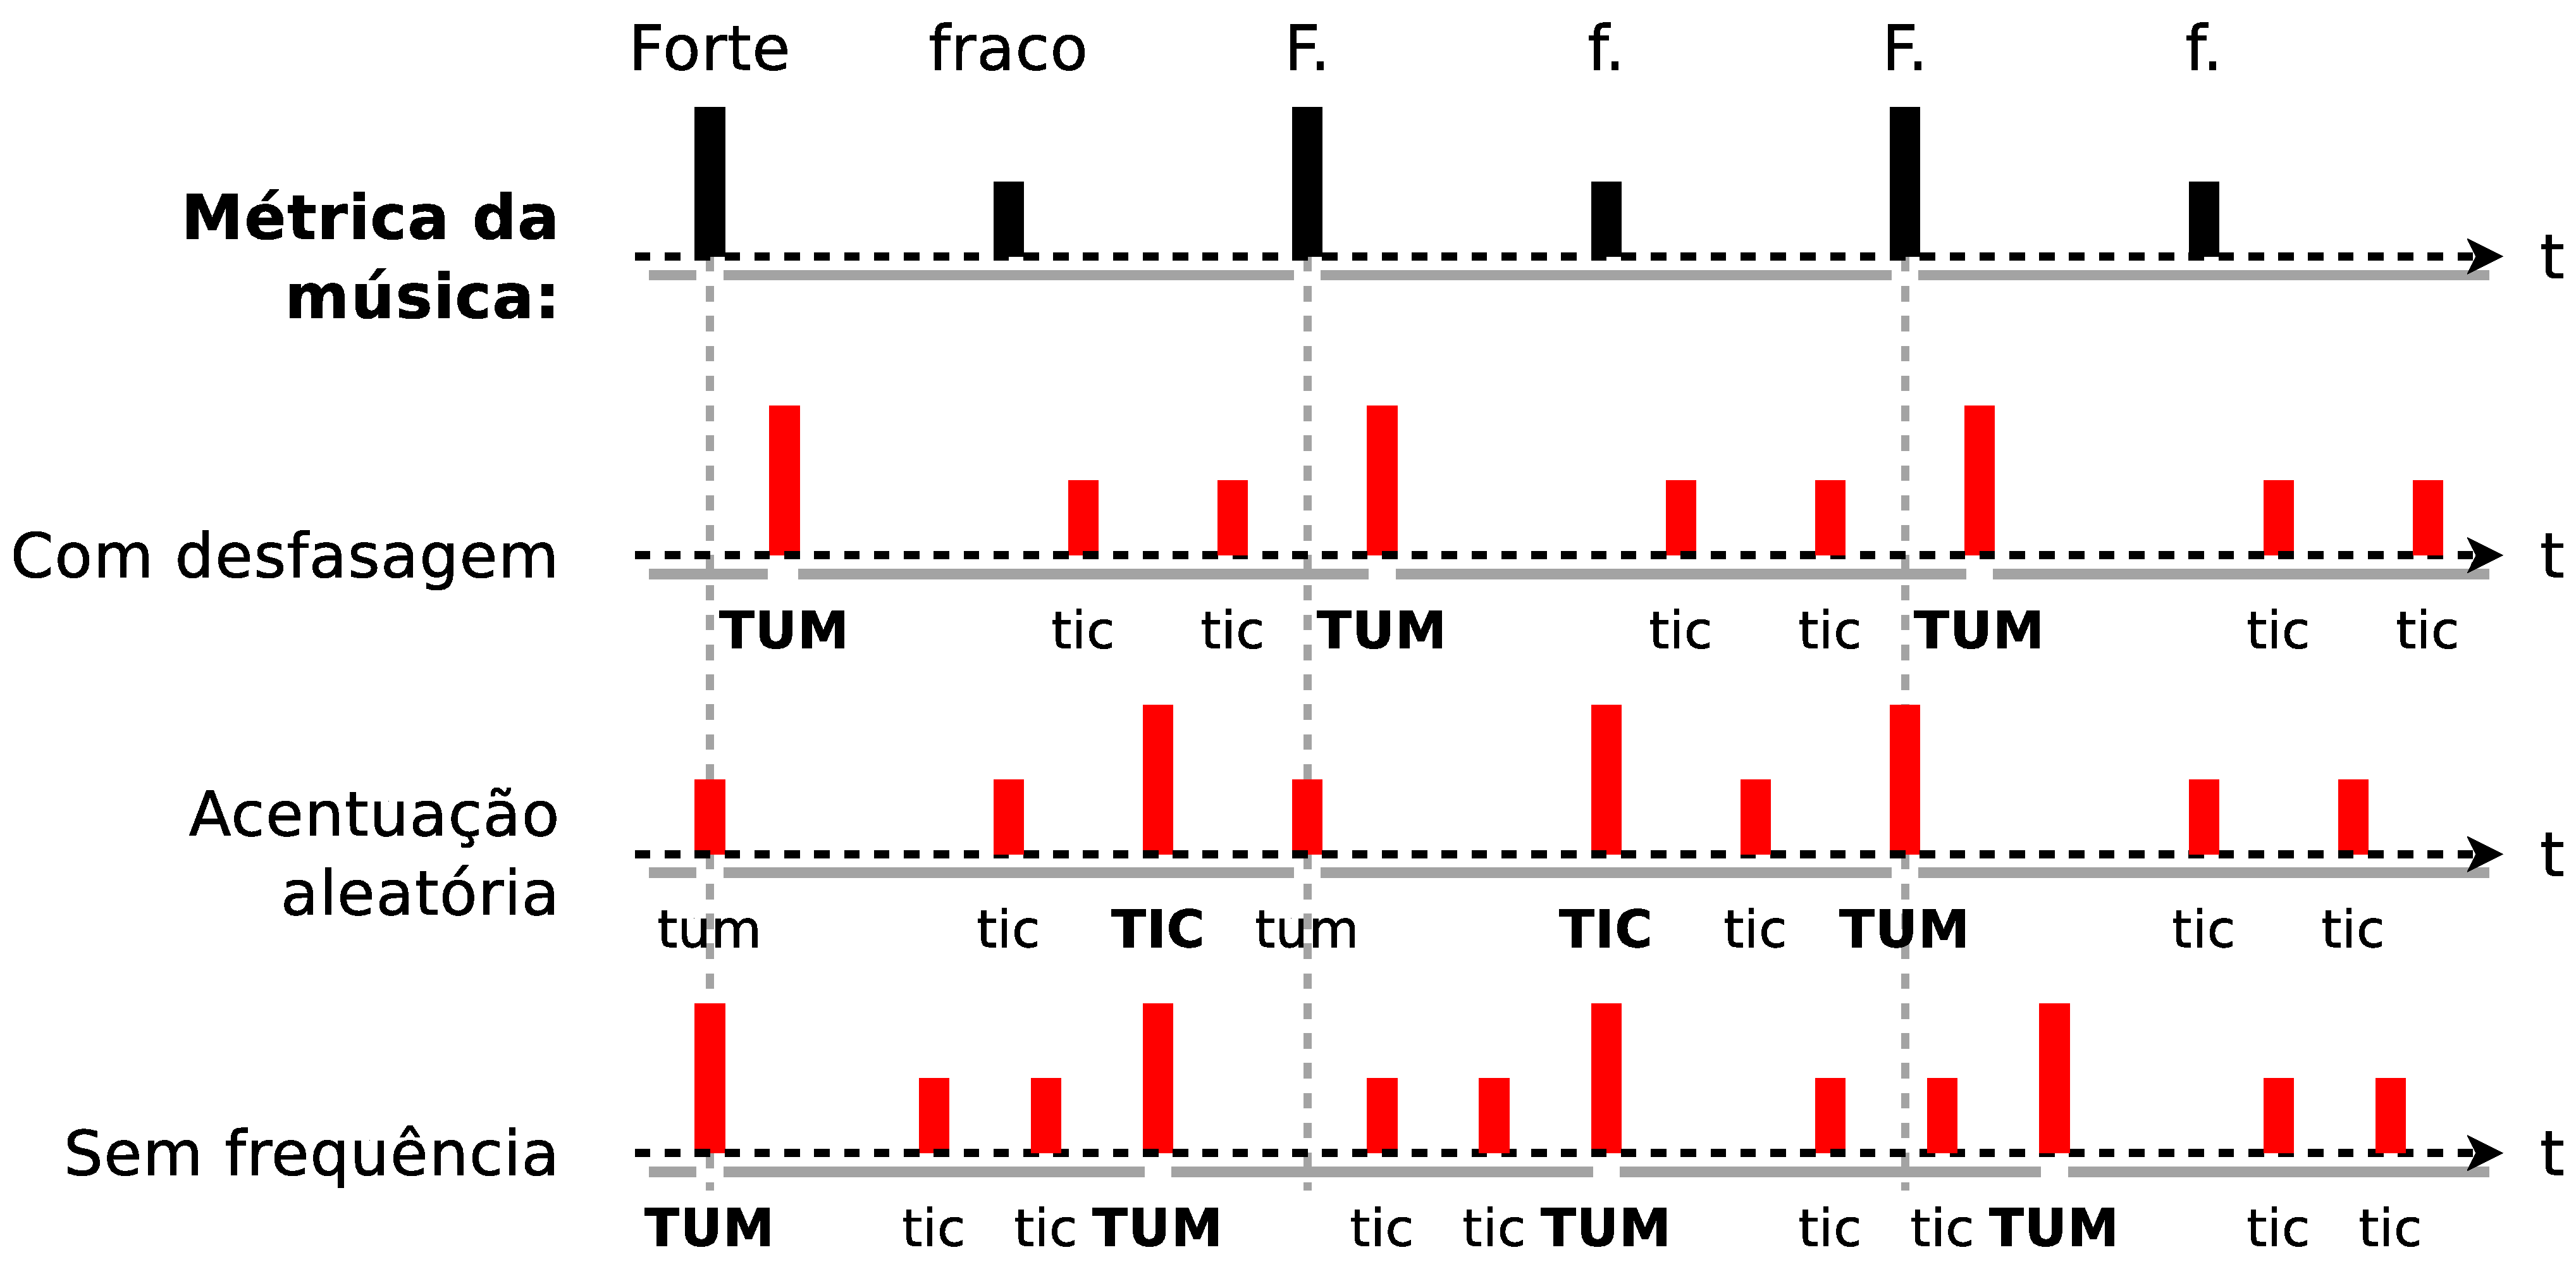
\includegraphics[width=0.99\textwidth]{chapters/cap-musicalidade/fora-do-ritmo-sem.eps}
    \caption{Dançando fora da métrica.}
    \label{fig:fora-do-ritmo-sem}
\end{figure}

Devemos ressaltar do Exemplo \ref{ex:fora-do-ritmo:2} que,
da mesma forma que na música, acentuar fora do acento métrico não é considerado um erro e sim um adorno; 
dançar não respeitando a acentuação métrica não necessariamente é considerado um erro,
e sim um enfeite. Mas, esta característica deve estar sobre o controle do dançarino,
e não ser algo solto à arbitrariedade, 
pois se nossa acentuação na dança tem pouca 
\hyperref[sec:musicalidadeinfmutua]{\textbf{informação mutua}} com o que está acontecendo na música, 
provavelmente o produto final (a dança) se perceberá com pouca musicalidade.  

